% Soubory musí být v kódování, které je nastaveno v příkazu \usepackage[...]{inputenc}

\documentclass[%        Základní nastavení
%  draft,    				  % Testovací překlad
  12pt,       				% Velikost základního písma je 12 bodů
  a4paper,    				% Formát papíru je A4
  oneside,      			% Jednostranný tisk
	%twoside,      			% Dvoustranný tisk (kapitoly a další důležité části tedy začínají na lichých stranách)
	unicode,						% Záložky a metainformace ve výsledném  PDF budou v kódování unicode
]{report}				    	% Dokument třídy 'zpráva', vhodná pro sazbu závěrečných prací s kapitolami

\usepackage[utf8]		  %	Kódování zdrojových souborů je UTF-8
	{inputenc}					% Balíček pro nastavení kódování zdrojových souborů

\usepackage[				% Nastavení geometrie stránky
	bindingoffset=10mm,		% Hřbet pro vazbu
	hmargin={25mm,25mm},	% Vnitřní a vnější okraj
	vmargin={25mm,34mm},	% Horní a dolní okraj
	footskip=17mm,			  % Velikost zápatí
	nohead,					      % Bez záhlaví
	marginparsep=2mm,		  % Vzdálenost marginálií
	marginparwidth=18mm,	% Šířka marginálií
]{geometry}

\usepackage{sectsty}
	%přetypuje nadpisy všech úrovní na bezpatkové, kromě \chapter, která je přenastavena zvlášť v thesis.sty
	\allsectionsfont{\sffamily}

\usepackage{graphicx} % Balíček 'graphicx' pro vkládání obrázků
											% Nutné pro vložení logotypů školy a fakulty

\usepackage[          % Balíček 'acronym' pro sazby zkratek a symbolů
	nohyperlinks				% Nebudou tvořeny hypertextové odkazy do seznamu zkratek
]{acronym}						
											% Nutné pro použití prostředí 'acronym' balíčku 'thesis'

\usepackage[
	breaklinks=true,		% Hypertextové odkazy mohou obsahovat zalomení řádku
	hypertexnames=false % Názvy hypertext. odkazů budou tvořeny nezávisle na názvech TeXu
]{hyperref}						% Balíček 'hyperref' pro sazbu hypertextových odkazů
											% Nutné pro použití příkazu 'pdfsettings' balíčku 'thesis'

\usepackage{pdfpages} % Balíček umožňující vkládat stránky z PDF souborů
                      % Nutné při vkládání titulních listů a zadání přímo
                      % ve formátu PDF z informačního systému

\usepackage{enumitem} % Balíček pro nastavení mezerování v odrážkách
  \setlist{topsep=0pt,partopsep=0pt,noitemsep} % konkrétní nastavení

\usepackage{cmap} 		% Balíček cmap zajišťuje, že PDF vytvořené `pdflatexem' je
											% plně "prohledávatelné" a "kopírovatelné"

%\usepackage{upgreek}	% Balíček pro sazbu stojatých řeckých písmem
											%% např. stojaté pí: \uppi
											%% např. stojaté mí: \upmu (použitelné třeba v mikrometrech)
											%% pozor, grafická nekompatibilita s fonty typu Computer Modern!
                      
%\usepackage{amsmath} %balíček pro sabu náročnější matematiky                 

\usepackage{dirtree}	% sazba adresářové struktury
                      % vhodné pro prezentaci obsahu elektronické přílohy (např. CD)

\usepackage[formats]{listings}	% Balíček pro sazbu zdrojových textů
\lstset{              % nastavení
%	Definice jazyka použitého ve výpisech
%    language=[LaTeX]{TeX},	% LaTeX
%	language={Matlab},		% Matlab
	language={C},           % jazyk C
    basicstyle=\ttfamily,	% definice základního stylu písma
    tabsize=2,			% definice velikosti tabulátoru
    inputencoding=utf8,         % pro soubory uložené v kódování UTF-8
		columns=fixed,  %fixed nebo flexible,
		fontadjust=true %licovani sloupcu
    extendedchars=true,
    literate=%  definice symbolů s diakritikou
    {á}{{\'a}}1
    {č}{{\v{c}}}1
    {ď}{{\v{d}}}1
    {é}{{\'e}}1
    {ě}{{\v{e}}}1
    {í}{{\'i}}1
    {ň}{{\v{n}}}1
    {ó}{{\'o}}1
    {ř}{{\v{r}}}1
    {š}{{\v{s}}}1
    {ť}{{\v{t}}}1
    {ú}{{\'u}}1
    {ů}{{\r{u}}}1
    {ý}{{\'y}}1
    {ž}{{\v{z}}}1
    {Á}{{\'A}}1
    {Č}{{\v{C}}}1
    {Ď}{{\v{D}}}1
    {É}{{\'E}}1
    {Ě}{{\v{E}}}1
    {Í}{{\'I}}1
    {Ň}{{\v{N}}}1
    {Ó}{{\'O}}1
    {Ř}{{\v{R}}}1
    {Š}{{\v{S}}}1
    {Ť}{{\v{T}}}1
    {Ú}{{\'U}}1
    {Ů}{{\r{U}}}1
    {Ý}{{\'Y}}1
    {Ž}{{\v{Z}}}1
}
\usepackage{listings}
%%%%%%%%%%%%%%%%%%%%%%%%%%%%%%%%%%%%%%%%%%%%%%%%%%%%%%%%%%%%%%%%%
%%%%%%      Definice informací o dokumentu             %%%%%%%%%%
%%%%%%%%%%%%%%%%%%%%%%%%%%%%%%%%%%%%%%%%%%%%%%%%%%%%%%%%%%%%%%%%%

% V tomto souboru se nastavují téměř veškeré informace, proměnné mezi studenty:
% jméno, název práce, pohlaví atd.
% Tento soubor je SDÍLENÝ mezi textem práce a prezentací k obhajobě -- netřeba něco nastavovat na dvou místech.

\usepackage[
%%% Z následujících voleb jazyka lze použít pouze jednu
  czech-english,		% originální jazyk je čeština, překlad je anglicky (výchozí)
  %english-czech,	% originální jazyk je angličtina, překlad je česky
  %slovak-english,	% originální jazyk je slovenština, překlad je anglicky
  %english-slovak,	% originální jazyk je angličtina, překlad je slovensky
%
%%% Z následujících voleb typu práce lze použít pouze jednu
  semestral,		  % semestrální práce (nesází se abstrakty, prohlášení, poděkování) (výchozí)
  %bachelor,			%	bakalářská práce
  %master,			  % diplomová práce
  %treatise,			% pojednání o disertační práci
  %doctoral,			% disertační práce
%
%%% Z následujících voleb zarovnání objektů lze použít pouze jednu
%  left,				  % rovnice a popisky plovoucích objektů budou zarovnány vlevo
	center,			    % rovnice a popisky plovoucích objektů budou zarovnány na střed (vychozi)
%
]{thesis}   % Balíček pro sazbu studentských prací


%%% Jméno a příjmení autora ve tvaru
%  [tituly před jménem]{Křestní}{Příjmení}[tituly za jménem]
% Pokud osoba nemá titul před/za jménem, smažte celý řetězec '[...]'
\author{Bc.\,Samuel\ Kopecký}{Bc.\,Michal\ Procházka}

%%% Identifikační číslo autora (VUT ID)
\butid{007}

%%% Pohlaví autora/autorky
% (nepoužije se ve variantě english-czech ani english-slovak)
% Číselná hodnota: 1...žena, 0...muž
\gender{0}

%%% Jméno a příjmení vedoucího/školitele včetně titulů
%  [tituly před jménem]{Křestní}{Příjmení}[tituly za jménem]
% Pokud osoba nemá titul před/za jménem, smažte celý řetězec '[...]'
\advisor[Ing.]{Michael}{Jurek}

%%% Jméno a příjmení oponenta včetně titulů
%  [tituly před jménem]{Křestní}{Příjmení}[tituly za jménem]
% Pokud osoba nemá titul před/za jménem, smažte celý řetězec '[...]'
% Nastavení oponenta se uplatní pouze v prezentaci k obhajobě;
% v případě, že nechcete, aby se na titulním snímku prezentace zobrazoval oponent, pouze příkaz zakomentujte;
% u obhajoby semestrální práce se oponent nezobrazuje (jelikož neexistuje)
% U dizertační práce jsou typicky dva až tři oponenti. Pokud je chcete mít na titulním slajdu, prosím ručně odkomentujte a upravte jejich jména v definici "VUT title page" v souboru thesis.sty.
%\opponent[doc.\ Mgr.]{Křestní}{Příjmení}[Ph.D.]

%%% Název práce
%  Parametr ve složených závorkách {} je název v originálním jazyce,
%  parametr v hranatých závorkách [] je překlad (podle toho jaký je originální jazyk).
%  V případě, že název Vaší práce je dlouhý a nevleze se celý do zápatí prezentace, použijte příkaz
%  \def\insertshorttitle{Zkác.\ náz.\ práce}
%  kde jako parametr vyplníte zkrácený název. Pokud nechcete zkracovat název, budete muset předefinovat,
%  jak se vytváří patička slidu. Viz odkaz: https://bit.ly/3EJTp5A
\title{Implementace postkvantového schématu kruhových podpisů}

%%% Označení oboru studia
%  Parametr ve složených závorkách {} je název oboru v originálním jazyce,
%  parametr v hranatých závorkách [] je překlad
\specialization[Teleinformatics]{Teleinformatika}

%%% Označení ústavu
%  Parametr ve složených závorkách {} je název ústavu v originálním jazyce,
%  parametr v hranatých závorkách [] je překlad
%\department[Department of Control and Instrumentation]{Ústav automatizace a měřicí techniky}
%\department[Department of Biomedical Engineering]{Ústav biomedicínského inženýrství}
%\department[Department of Electrical Power Engineering]{Ústav elektroenergetiky}
%\department[Department of Electrical and Electronic Technology]{Ústav elektrotechnologie}
%\department[Department of Physics]{Ústav fyziky}
%\department[Department of Foreign Languages]{Ústav jazyků}
%\department[Department of Mathematics]{Ústav matematiky}
%\department[Department of Microelectronics]{Ústav mikroelektroniky}
%\department[Department of Radio Electronics]{Ústav radioelektroniky}
%\department[Department of Theoretical and Experimental Electrical Engineering]{Ústav teoretické a experimentální elektrotechniky}
\department[Department of Telecommunications]{Ústav telekomunikací}
%\department[Department of Power Electrical and Electronic Engineering]{Ústav výkonové elektrotechniky a elektroniky}

%%% Označení fakulty
%  Parametr ve složených závorkách {} je název fakulty v originálním jazyce,
%  parametr v hranatých závorkách [] je překlad
%\faculty[Faculty of Architecture]{Fakulta architektury}
\faculty[Faculty of Electrical Engineering and~Communication]{Fakulta elektrotechniky a~komunikačních technologií}
%\faculty[Faculty of Chemistry]{Fakulta chemická}
%\faculty[Faculty of Information Technology]{Fakulta informačních technologií}
%\faculty[Faculty of Business and Management]{Fakulta podnikatelská}
%\faculty[Faculty of Civil Engineering]{Fakulta stavební}
%\faculty[Faculty of Mechanical Engineering]{Fakulta strojního inženýrství}
%\faculty[Faculty of Fine Arts]{Fakulta výtvarných umění}
%
%Nastavení logotypu (v hranatych zavorkach zkracene logo, ve slozenych plne):
\facultylogo[logo/FEKT_zkratka_barevne_PANTONE_CZ]{logo/UTKO_color_PANTONE_CZ}

%%% Rok odevzdání práce
\graduateyear{2022}

%%% Datum obhajoby (uplatní se pouze v prezentaci k obhajobě)
\date{08.\,12.\,2022} 

%%% Místo obhajoby
% Na titulních stránkách bude automaticky vysázeno VELKÝMI písmeny (pokud tyto stránky sází šablona)
\city{Brno}
  % do tohoto souboru doplňte údaje o sobě, druhu práce, názvu...

%%%%%%%%%%%%%%%%%%%%%%%%%%%%%%%%%%%%%%%%%%%%%%%%%%%%%%%%%%%%%%%%%%%%%%%%

%%%%%%%%%%%%%%%%%%%%%%%%%%%%%%%%%%%%%%%%%%%%%%%%%%%%%%%%%%%%%%%%%%%%%%%%
%%%%%%     Nastavení polí ve Vlastnostech dokumentu PDF      %%%%%%%%%%%
%%%%%%%%%%%%%%%%%%%%%%%%%%%%%%%%%%%%%%%%%%%%%%%%%%%%%%%%%%%%%%%%%%%%%%%%
%% Při načteném balíčku 'hyperref' lze použít příkaz '\pdfsettings':
\pdfsettings
%  Nastavení polí je možné provést také ručně příkazem:
%\hypersetup{
%  pdftitle={Název studentské práce},    	% Pole 'Document Title'
%  pdfauthor={Autor studenstké práce},   	% Pole 'Author'
%  pdfsubject={Typ práce}, 						  	% Pole 'Subject'
%  pdfkeywords={Klíčová slova}           	% Pole 'Keywords'
%}
%%%%%%%%%%%%%%%%%%%%%%%%%%%%%%%%%%%%%%%%%%%%%%%%%%%%%%%%%%%%%%%%%%%%%%%

\pdfmapfile{=vafle.map}

%%%%%%%%%%%%%%%%%%%%%%%%%%%%%%%%%%%%%%%%%%%%%%%%%%%%%%%%%%%%%%%%%%%%%%%
%%%%%%%%%%%       Začátek dokumentu               %%%%%%%%%%%%%%%%%%%%%
%%%%%%%%%%%%%%%%%%%%%%%%%%%%%%%%%%%%%%%%%%%%%%%%%%%%%%%%%%%%%%%%%%%%%%%
\begin{document}
\pagestyle{empty} %vypnutí číslování stránek

\maketitle
\cleardoublepage\pagestyle{plain} 

%% Vysázení obsahu
\tableofcontents

\chapter*{Úvod}
\phantomsection
\addcontentsline{toc}{chapter}{Úvod}

Kruhové podpisy jsou typy digitálních podpisů, které zajišťují anonymitu člena podepisující skupiny a zároveň potvrzují, že podpis je opravdu od člena dané skupiny. Rychlost rozšifrování zprávy a odhalení původce zprávy ze skupiny záleží na použitých protokolech k~podepisování. Tento typ podepisování se často používá u~kryptoměn (např. ShadowCash, Monero) k~ověřování plateb a zároveň anonymitě člověka, který platí.

S vývojem kvantových počítačů je potřeba začít vylepšovat současnou kryptografii, která není odolná vůči kvantovým počítačům. Jedním z~kvantově odolných kryptografických primitiv je kryptografie založená na mřížkách, která je popsána v~teoretické části. Toto kryptografické primitivum společně s~kruhovými podpisy jsme společně zkoumali jak fungují a následně implementovali řešení, které je popsáno v~praktické části.


\chapter{Teorie}
Teoretická část práce se skládá ze~ dvou částí. První část věnuje popisu fungování kruhových podpisů obecně a druhá část se věnuje kryptografii založenou na mřížkách, které jsou odolné vůči kvantové kryptografii.

\section{Kruhové podpisy}

Metoda kruhového podpisu byla vytvořena v~roce 2001 skupinou Ronald L. Rivest, Adi Shamir a Yael Tauman. Výhoda kruhových podpisů je, že poskytují anonymitu členům skupiny při podepisování zpráv, dále jejich nezapomenutelnost a odolnost vůči kolizím. Během podepisování zprávy nejsme schopni zjistit, kdo jako první podepsal zprávu a kdo jako poslední, protože se jednotlivé zprávy na sebe odkazují a jeví se jako dokonalý kruh. Ani lidé z~podepisující skupiny neví, kteří další členové a v~jakém pořadí podepsali zprávu.

V~kruhovém podpisu má každý člen vlastní pár asymetrických klíčů (tedy soukromého a veřejného klíče). V~případě, že by jeden člen skupiny chtěl podepsat zprávu, musí vybrat členy skupiny, kteří zprávu podepíší (nemusí to být všichni členové skupiny, ale čím méně členů tím vyšší pravděpodobnost tipnutí si původci zprávy) a následně vykonat následující kroky. 

Vytvořit si náhodnou inicializační hodnotu \emph{u}. Vytvořit si šifrovací klíč z hashe původní zprávy $E = H(\mathrm{zpráva})$. Vytvoří si původní hodnotu \emph{v}, ze šifrovacího klíče a inicializační hodnoty $v = E(u)$, kterou bude využita dále. Vytvořit podepsání zprávy dalšími členy skupiny a to vytvořením náhodné hodnoty $x_i$, které umocníme veřejným klíčem člena skupiny $v = E(x_1^{pk_1})$ a použijeme exkluzivní disjunkci s~původní hodnotou \emph{v}. Tento krok se opakuje dokud nezbývá podpis pouze uživatele, který tuto operaci začal. Poslední krok vykoná uživatel vypočtením poslední hodnoty \emph{v}~pomocí exkluzivní disjunkce s~inicializační hodnotou, kde výsledek umocní na svůj soukromý klíč $v = E(u \oplus v)^{sk}$. Po vytvoření všech potřebných hodnot uživatel odešle původní zprávu, hodnotu $v$, včetně vygenerovaných náhodných $x_i$ hodnot uživatelů a veřejné klíče uživatelů.

Pro ověření zprávy, že opravdu pochází ze skupiny z~jaké se vydává. Uživatel pro ověření použije stejné kroky při šifrování kromě poslední kroku, který je jemně pozměněn. V~posledním kroku bude poslední hodnotu umocňovat veřejným klíče jednoho z~podepisujících (nezáleží na pořadí v~jakém ověřující člověk informace potřebné k~ověření) $v = E[(u \oplus v)^{sk}]^{pk}$, díky matematice v~pozadí těchto operací se ověří díky XOR operacím, že se jedná opravdu o~podpis některého z~uživatelů skupiny \cite{Buchanan}.

\begin{figure}[htbp]
  \centering
  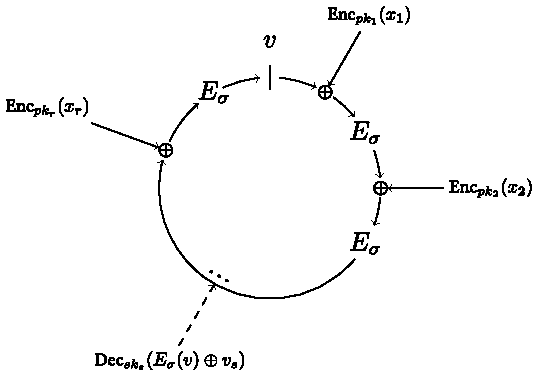
\includegraphics[width=0.7\textwidth]{img/ring_signature.pdf}
  \caption{Ukázka kruhového podpisu \cite{Ring signature picture}.}
  \label{Ring signature}
\end{figure}


\section{Kryptografie založená na mřížkách}

Metoda kterou jsme implementovali v této práci využívá mřížky, což jsou množiny bodů v n-rozměrném prostoru uspořádány periodicky. Využívají dvou matematických problémů, které jsou imunní vůči kvantovým počítačům. Máme soubor lineárně nezávislých vektorů, které generují mřížku.

Prvním problémem je problém nejkratšího vektoru (Shortest Vector Problem - SVP). Problematikou je hledáním nejkratšího vektoru báze, který patří do dané mřížky. Součásti problému je také nalezení co nejmenšího vektoru, který není nulový. Druhým problémem je nalezení nejbližšího vektoru, což je spojeno s~nalezením nejbližšího libovolného vektoru v~mřížce. Zde je možné, aby nalezený vektor byl nulový a zároveň byl nejblíže zvolenému bodu (Closest vector problem - CVP). Naše vybrané schéma právě využívá problém nejkratšího vektoru (SVP).


\section{Jiné druhy podpisů}

Existuje spousta různých druhů post kvantových algoritmů pro samotné podpisy. Níže uvedené jsou často používané na podepisování. 

\begin{itemize}
  \item Hash-and-sign,
  \item Bimodal Lattice Signature Scheme (BLISS),
  \item Goldreich-Goldwasser-Halevi (GGH),
  \item NTRU Signature Algorithm,
\end{itemize}

\hfill

Zároveň jsme uvedené algoritmy posloužili jako inspirace pro námi vybraného algoritmu, který byl v~této práci implementován. Post kvantová kryptografie není zase až tak rozšířená takže počet kruhových post kvantových podpisu je menší. Zde jsou uvedeny všechny ostatní kruhové podpisy které jsme zvážili na implementaci.

\begin{itemize}
  \item Lattice-based Linkable Ring Signature with Co-Signing (L2RS-CS) \cite{Torres2020}.
\end{itemize}


\begin{figure}[htbp]
  \centering
  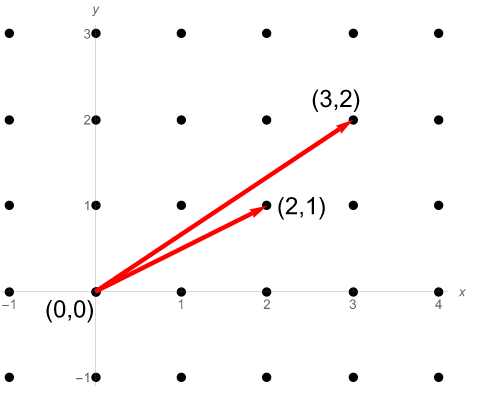
\includegraphics[width=0.7\textwidth]{img/mrizky.png}
  \caption{Ukázka kryptografie na mřížkách \cite{Mrizky picture}.}
  \label{lattice}
  \label{Ring signature}
\end{figure}


\newcommand{\param}[2]{\textit{#1}\,--\,#2\,--\,}
\newcommand{\paramnott}[2]{#1\,--\,#2\,--\,}

\chapter{Praktická část}
Praktická část práce se skládá z~dvou častí. První část je implementace samotného protokolu L2RS a~druhá část je ukázková aplikace která využívá implementaci protokolu. Sekce níže popisují jednotlivé části práce.

\section{Protokol L2RS}
Protokol L2RS je implementovaný v jazyku Python a jako jedinou knihovnu využívá \texttt{numpy}. Parametre pro protokol bili zvolené následovně
\begin{itemize}
  \item \param{q}{12289}modulus pre koeficienty v polynomech,
  \item \param{n}{512}počet koeficientů v polynomech,
  \item \param{m}{6}počet polynomů vo vektoru polynomů,
  \item \paramnott{$\sigma$}{283754}standardní guassova odchylka,
  \item \paramnott{$\gamma$}{13.6}hustota privátního klíče.
\end{itemize}
Tyto parametre bily zvolené aby splňovali bezpečnostní úroveň \texttt{III} protokolu. Vytváření podpisu trvá průměrně 43\,ms a ověření průměrně 38\,ms při výše opomenutých parametrech. Rychlost podpisu a ověření je samozřejmé závislá na parametrech stroje na kterém byli testované. Tyto časy byli měřené na procesoru AMD Ryzen 3600 z frekvencí jádra 3.6\,GHz.

V tabulce \ref{sizes} je možné vidět velkosti jednolitých konstrukcí jako veřejný nebo~privátní klíč. Velkosti podpisu jsou lineárně závislé na počtu uživatelů který se zúčastňují podpisu. Velkost podpisu se dá jednoduše vypočítat podle rovnice
\begin{equation}
  S=1792+w*m*896
\end{equation}
kde $w$ označuje počet uživatelů a $m$ je počet polynomech ve jedním vektoru polynomu.

\begin{table}[htbp]
  \centering
  \caption{Velkosti konstrukcí podpisu}
  \begin{tabular}{|l|c|c|}
    \hline
    Typ              & Počet uživatelů & Velkost (B) \\
    \hline
    Veřejný klíč     & -               & 896         \\
    Privátní klíč    & -               & 4480        \\
    Veřejný parametr & -               & 8960        \\
    Podpis           & 1               & 7168        \\
    Podpis           & 2               & 12544       \\
    Podpis           & 5               & 28672       \\
    \hline
  \end{tabular}
  \label{sizes}
\end{table}


\section{Ukázková aplikace}
Součást práce je taktéž ukázková aplikace která vyváří komunikaci mezi uživateli který jsou schopný ověřovat vytvořené podpisy. Aplikace se skládá z třech částí: \textbf{proxy server}, \textbf{podpisovatel} a \textbf{ověřovatel}. Jako je možné vidět na obrázku \ref{network_diagram}, proxy server přeposílá generovaný podpis všem připojeným ověřovatelům. Taky se~stará o~generovaní veřejných parametrů které posílá na vyžádaní uživatelům. Uživatel může být ověřovatel nebo podpisovatel. 

Podpis se generuje jenom jedním podpisovatelem z využitím soukromého klíče, veřejných parametru a veřejných klíčů všech účastníku. Veřejné klíče jsou zasílané uživateli proxy serveru když se poprvé připojí a vygenerují si soukromý a veřejný klíč. Proxy server stejně jako veřejné parametre poskytuje i posbírané veřejné klíče na vyžádaní. Když podpisovatel zašle vygenerovaný podpis na správu která byla zadaná, je přeposlána všem uživatelům aby ji mohly ověřit pomocí veřejných parametru, veřejných klíčů všech účastníku a originální správy.

\begin{figure}[htbp]
  \centering
  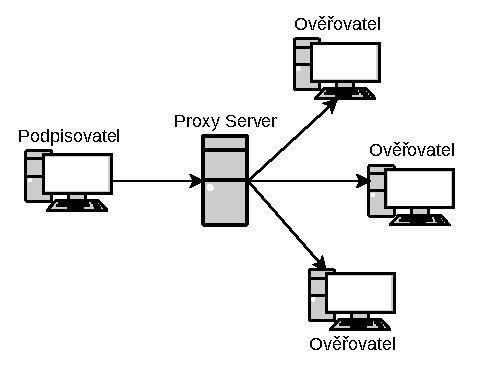
\includegraphics[width=0.65\textwidth]{img/network_diagram.pdf}
  \caption{Sítová komunikace}
  \label{network_diagram}
\end{figure}

Stanice si mezi sebou správy vyměňují pomocí protokolu TCP s jednoduchou aplikační hlavičkou, který formát je možné vidět na obrázků \ref{header}. Políčko typ správy označuje co je obsahem správy. Typy správ jsou následovné:
\begin{itemize}
  \item \texttt{NEED\_PUB\_PARAMS} -- uživatel požaduje veřejné parametre,
  \item \texttt{PUB\_PARAMS} -- server posílá veřejné parametre,
  \item \texttt{MY\_PUB\_KEY} -- uživatel zasílá svůj veřejný klíč,
  \item \texttt{NEED\_PUB\_KEYS} -- uživatel požaduje veřejné klíče všech uživatelů,
  \item \texttt{PUB\_KEYS} -- server posílá veřejné klíče všech uživatelů,
  \item \texttt{SIGNATURE} -- uživatel nebo server zasílá podpis na ověření.
\end{itemize}

\begin{figure}[htbp]
  \centering
  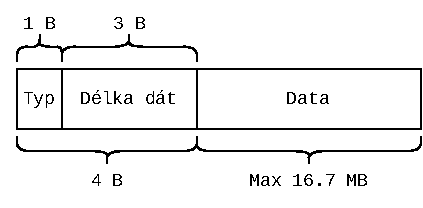
\includegraphics[width=0.7\textwidth]{img/header.pdf}
  \caption{Aplikační hlavička}
  \label{header}
\end{figure}

\subsection{Návod na použití}
Program používá přepínače na jeho ovládaní. Spuštění je možné ve Windows powershellu, WSL (Windows Subsystem for Linux) a libovolné linux distribuci. Program byl testovaný na verzi \texttt{Python 3.10.7}. Návod na spuštění je následovný. Jako první je potřeba nainstalovat potřebné balíčky pomocí souboru \texttt{requirements.txt} který se nachází v odevzdaném kódu:
\begin{itemize}
  \item \texttt{pip install -r requirements.txt}
\end{itemize}
Spustit \textbf{pouze jeden} proxy server:
\begin{itemize}
  \item \texttt{./ring\_sig.py -sp}
\end{itemize}
Spustit \textbf{pouze jednoho} podpisovatele:
\begin{itemize}
  \item \texttt{./ring\_sig.py -c -s}
\end{itemize}
Spustit \textbf{maximum 255} ověřovatelů:
\begin{itemize}
  \item \texttt{./ring\_sig.py -c -v}
\end{itemize}
Dále stačí jednom zadat text který bude podepsaní a ověřený u každého ověřovatele. Jako předvolené nastavení používá program port \textbf{3000} pro komunikaci. Tento port je možné změnit pomocí přepínače \texttt{-p}.
\begin{itemize}
  \item \texttt{./ring\_sig.py -p [PORT]}
\end{itemize}
Všechny dostupné přepínače se dají zobrazit pomocí:
\begin{itemize}
  \item \texttt{./ring\_sig.py -h}
\end{itemize}
Dále je možné zobrazit jednotlivé parametre které sou použité pro protokol L2RS a~sítovou komunikaci:
\begin{itemize}
  \item \texttt{./ring\_sig.py -i}
\end{itemize}




\chapter*{Závěr}
\phantomsection
\addcontentsline{toc}{chapter}{Závěr}
Shrnutí semestrálního projektu.


\begin{thebibliography}{99}

\bibitem{lit1}MPC-CT3 semestral project \textit{VUT} [online]. [cit. 2022-09-27]. Dostupné z: \url{https://www.vut.cz/}

\end{thebibliography}

%% Konec dokumentu
\end{document}
